% =====================================================================
% Modelo para Relatório Parcial de Iniciação Científica (em Português)
% Prof. Vítor E. Silva Souza - NEMO/UFES :: DI/UFES :: PPGI/UFES
%
% Baseado no modelo fornecido pela PRPPG/UFES:
% https://prppg.ufes.br/programa-institucional-de-ic-piic
%
% This work may be distributed and/or modified under the conditions of 
% the LaTeX Project Public License, either version 1.3 of this license 
% or (at your option) any later version. The latest version of this 
% license is in http://www.latex-project.org/lppl.txt.
% =====================================================================
\documentclass[10pt, a4paper]{article}

\usepackage[pdftex]{graphicx,color}
\usepackage[dvipsnames]{xcolor,colortbl}
\usepackage[hidelinks]{hyperref}
\usepackage{anysize}
\usepackage{graphicx}
\usepackage[utf8]{inputenc}
\usepackage[portuges,brazilian]{babel}
\usepackage{fancyhdr}
\usepackage{ifthen}
\usepackage{array}
\usepackage{natbib}
%\usepackage{ tipa }
\usepackage{amssymb}
\usepackage{amsmath}
%\usepackage[usenames,dvipsnames]{xcolor} %to allow for color changes
%\definecolor{light-gray}{gray}{0.80} % defines the colour.
%\usepackage{cite} % to allow line breaks inside citations

%% Para redução de espaço entre os itens da bibliografia
	\let\oldbibliography\thebibliography
	\renewcommand{\thebibliography}[1]{\oldbibliography{#1}
	\setlength{\itemsep}{0pt}}

\usepackage{helvet}
\renewcommand{\familydefault}{\rmdefault}

\usepackage{enumerate}
\usepackage{adjustbox}

\usepackage{parskip}% http://ctan.org/pkg/parskip
\setlength{\parindent}{0pt}

\linespread{1.25}

\usepackage{titlesec}

\titleformat{\section}
  {\normalfont\Large\bfseries}{\thesection}{1em}{}[{\titlerule[0.8pt]}]

\newcommand{\mnras}{Mon. Not. R. Astron. Soc.}
\newcommand{\aap}{Astronomy $\&$ Astrophysics}
\newcommand{\apjs}{ApJS}
\newcommand{\apj}{Astrophys. J.}
\newcommand{\apjl}{Astrophys. J. Letters}
\newcommand{\aj}{Astron. J.}
\newcommand{\pasa}{PASA}
\newcommand{\nat}{Nature}

\usepackage{mathptmx}
\usepackage{tabularx}

\usepackage{caption}
\usepackage{subcaption}

\usepackage{newfloat}
\DeclareFloatingEnvironment[name={Gráfico}]{grafico}
\DeclareFloatingEnvironment[name={Quadro}]{quadro}

\usepackage{enumitem}
\setlist[enumerate]{nosep}

% Colorinlistoftodos package: to insert colored comments so authors can collaborate on the content.
\usepackage[colorinlistoftodos, textwidth=20mm, textsize=footnotesize]{todonotes}
\newcommand{\aluno}[1]{\todo[author=\textbf{Aluno},color=green!30,caption={},inline]{#1}}
\newcommand{\professor}[1]{\todo[author=\textbf{Professor},color=red!30,caption={},inline]{#1}}

% Permite usar o comando \hl{} para evidenciar texto com fundo amarelo. Útil para chamar atenção a itens a fazer.
\usepackage{soulutf8}

%\marginsize{left}{right}{top}{bottom}
\marginsize{30mm}{20mm}{30mm}{20mm}

%\renewcommand{\arraystretch}{1.5}


\usepackage{fancyhdr}
\usepackage{afterpage}
\pagestyle{fancy}
\fancyhf{} % clear all fields
\fancyhead[R]{\color{Gray} Universidade Federal do Espírito Santo\\ Programa Institucional de Iniciação Científica\\ Relatório Parcial de Pesquisa\\ {\color{Red} Área do Conhecimento (CNPq)}}
\setlength{\headheight}{40pt}
\renewcommand{\headrulewidth}{0pt}

%\pagenumbering{arabic}

% Pacote xspace: para colocar espaços no final das macros quando necessário.
\usepackage{xspace}

\usepackage{tikz}
\newcommand{\smiley}{\tikz[baseline=-0.75ex,black]{
		\draw circle (1.8mm);
		\node[fill,circle,inner sep=0.5pt] (left eye) at (135:0.8mm) {};
		\node[fill,circle,inner sep=0.5pt] (right eye) at (45:0.8mm) {};
		\draw (-145:0.9mm) arc (-120:-60:1.5mm);
	}
}
\newcommand{\frownie}{\tikz[baseline=-0.75ex,black]{
		\draw circle (1.8mm);
		\node[fill,circle,inner sep=0.5pt] (left eye) at (135:0.8mm) {};
		\node[fill,circle,inner sep=0.5pt] (right eye) at (45:0.8mm) {};
		\draw (-145:0.9mm) arc (120:60:1.5mm);
	}
}
\newcommand{\neutranie}{\tikz[baseline=-0.75ex,black]{
		\draw circle (1.8mm);
		\node[fill,circle,inner sep=0.5pt] (left eye) at (135:0.8mm) {};
		\node[fill,circle,inner sep=0.5pt] (right eye) at (45:0.8mm) {};
		\draw (-135:0.9mm) -- (-45:0.9mm);
	}
}


% Definição de macros.
\newcommand{\java}{Java\texttrademark\xspace}



\begin{document}

\afterpage{\cfoot{\thepage}}



\begin{center}
 {\Large \bf  {\color{Red} Título do Subprojeto de Iniciação Científica -- PIIC/UFES}}
 \end{center}

\vspace{.5cm}


\bgroup
\def\arraystretch{1.3}
\begin{tabularx}{\textwidth}{|>{\columncolor{gray!25}}l|X|}
\hline
{\bf Edital:} & Edital PIIC 20\_\_ /20\_\_ \\
\hline
{\bf Área do Conhecimento (CNPq):} &  \\
\hline
{\bf Subárea do Conhecimento (CNPq):} &  \\
\hline
{\bf Título do Projeto:} &  \\
\hline
{\bf Título do Subprojeto:} &  \\
\hline
{\bf Professor(a) Orientador(a):}&   \\
\hline
{\bf Estudante:} &   \\
\hline
\end{tabularx}
\egroup

\vspace{.5cm}

%\bigskip


%%%%%%%%%%%%%%%%%%%%%%%%%%%%%
\section{Introdução}
\label{sec-intro}

O Relatório Parcial é individual e deve ser escrito pelo bolsista/voluntário de iniciação científica, sob a supervisão do seu orientador. O relatório deverá ser enviado pelo orientador através do sistema do Programa Institucional de Iniciação Científica no SAPPG até a data limite estabelecida no edital. O \textit{link} para envio do relatório está disponível no sistema do PIIC a partir do dia de início de envio estabelecido no edital. 

O envio do Relatório Parcial após a data limite estabelecida implicará na suspensão do pagamento da bolsa de Iniciação Científica, como previsto no subitem 7.1 do edital do PIIC, podendo ainda implicar em impedimento de participação do(a) orientador(a) do(a)(s) bolsista(a)(s) ou voluntário(a)(s) em futuras edições do PIIC, conforme previsto no inciso V do Art. 11º do Regulamento Geral do PIIC, disponível no site da Pró-Reitoria de Pesquisa e Pós-Graduação (PRPPG).

Este documento deve ser utilizado como modelo para a elaboração do Relatório Parcial de Pesquisa no âmbito do Programa Institucional de Iniciação Científica (PIIC) da UFES, que deve ser composto das seguintes seções: Introdução, Materiais e Métodos, Resultados e Discussão, Atividades Realizadas e Metas Futuras, e Referências Bibliográficas. 

O texto do Relatório Parcial de Pesquisa deve ser preparado considerando que todas as seções que compõem o documento não excedam seus limites, em formato A4 com margens de 3 cm (esquerda e superior) e de 2 cm (direita e inferior), usando fonte Times New Roman, tamanho 10, com espaçamento entre linhas de 1,5, sem recuo na primeira linha de cada parágrafo e com alinhamento justificado. Já os títulos das seções também devem utilizar a fonte Times New Roman, mas com tamanho 12. Por fim, o cabeçalho de todas as páginas deve ser mantido de acordo com a formatação deste modelo (Times New Roman, tamanho 9, alinhado à direita), sendo que deve-se alterar para a cor preta e descrever a Área do Conhecimento do projeto segundo o Conselho Nacional de Desenvolvimento Científico e Tecnológico (CNPq) na quarta linha do cabeçalho, isto é, Ciências Exatas e da Terra, Ciências Biológicas, Engenharias, Ciências da Saúde, Ciências Agrárias, Ciências Sociais Aplicadas, Ciências Humanas ou Linguística, Letras e Artes. O título do Subprojeto de Iniciação Científica deve ser inserido no lugar de ``Título do Subprojeto de Iniciação Científica – PIIC/Ufes'' e sua cor, também trocada para a preta.

A linguagem utilizada ao longo do trabalho deve ser técnica e impessoal, uma vez que se trata de um trabalho acadêmico. Deve-se evitar o uso de gírias e de termos de linguagem coloquial, bem como o uso das primeiras pessoas do singular e do plural (fiz ou fizemos...; obtive ou obtivemos...), e priorizar a estrutura passiva (fez-se...; foram obtidos...). 

O conteúdo de cada seção deve estar de acordo com as recomendações descritas neste modelo. Na Introdução, o autor deve apresentar, de forma concisa, uma contextualização do tema de sua pesquisa, mostrando sua relevância, justificando o tema escolhido, e descrevendo claramente a sua pergunta ou seu problema de pesquisa. Deve-se também ressaltar a ligação do Subprojeto de Iniciação Científica com o Projeto de Pesquisa ao qual está vinculado. Esta seção deve conter, \textbf{no máximo, 30 linhas}.



%%%%%%%%%%%%%%%%%%%%%%%%%%%%%
\section{Materiais e Métodos}
\label{sec-metodo}

Nesta seção devem ser descritos, de maneira sucinta, \textbf{em até 30 linhas}, o detalhamento da metodologia utilizada no decorrer da pesquisa executada pelo discente no primeiro semestre de vinculação ao PIIC/UFES, bem como os procedimentos de trabalho adotados, os materiais que foram utilizados, o tratamento da informação realizado e o procedimento estatístico aplicado, se for o caso. Esta seção deve, entretanto, além de detalhar os aspectos da metodologia empregada nas atividades especificamente executadas pelo estudante, apresentar sua relação com o Projeto de Pesquisa ao qual o Subprojeto de Iniciação Científica está vinculado.



%%%%%%%%%%%%%%%%%%%%%%%%%%%%%
\section{Resultados e Discussão}
\label{sec-resultados}

Esta seção deve explicitar, \textbf{em até 30 linhas}, os principais resultados obtidos no decorrer da pesquisa executada pelo discente no primeiro semestre de vinculação ao PIIC/UFES. Em todo o relatório, ilustrações (figuras, gráficos, fotos, fluxogramas, quadros e etc.) e tabelas podem também ser incluídas e devem ser utilizadas a fim de explicar ou complementar visualmente o texto. Deve-se destacar que tais ilustrações ou tabelas não são computadas como linhas do texto. Segundo a NBR 15287:2011, ``a ilustração deve ser citada no texto e inserida o mais próximo possível do trecho a que se refere.''~\citep[p. 8]{abnt:nbr15287}. Cabe ressaltar que a citação, no texto, sempre deve preceder a ilustração ou a tabela. Estes elementos devem estar centralizados na página, com identificação na parte superior e a indicação da fonte consultada (elemento obrigatório, mesmo que seja “produção do próprio autor”), com legenda, notas e outras informações necessárias à sua compreensão (se houver), na parte inferior (alinhados à borda esquerda da ilustração e limitados pela borda direita da mesma), como mostram a Figura~\ref{fig-exemplo} e o Gráfico~\ref{graf-exemplo}.

\begin{figure}[h!]
	\centering
	\caption{(a) Fotografia do modelo de edificação utilizado no experimento e (b) representação esquemática do comportamento do escoamento sobre a edificação}
	\label{fig-exemplo}
	\begin{subfigure}[b]{0.45\textwidth}
		\centering
		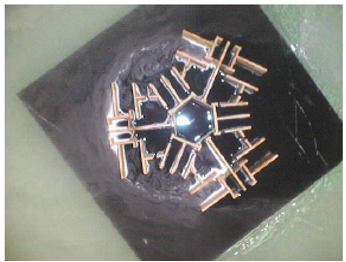
\includegraphics[width=\textwidth]{fig-exemploA}
		\caption{}
		\label{fig-exemploA}
	\end{subfigure}
	\hfill
	\begin{subfigure}[b]{0.45\textwidth}
		\centering
		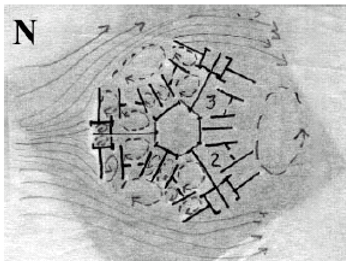
\includegraphics[width=\textwidth]{fig-exemploB}
		\caption{}
		\label{fig-exemploB}
	\end{subfigure}
	\caption*{Fonte: \cite{toledo-pereira:clacs2004}.}
\end{figure}

\begin{grafico}[h!]
	\centering
	\caption{Consumo final de energia por fonte no Brasil em 2011}
	\label{graf-exemplo}
	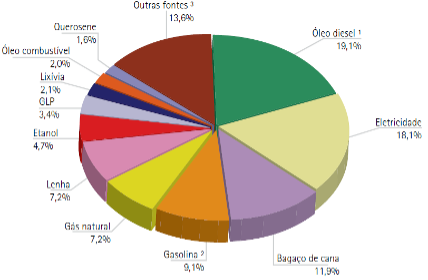
\includegraphics[width=.75\textwidth]{graf-exemplo}	
	\caption*{Fonte: \cite{epe:ben2011}.}
\end{grafico}

As tabelas e os quadros, apesar de possuírem certa semelhança entre si, diferenciam-se não apenas no formato exigido, mas também pelo conteúdo que exibem:

\begin{enumerate}[label=\alph*)]
	\item um quadro apresenta informações ou resultados qualitativos, ou seja, em forma de texto, mesmo que este empregue números;
	\item uma tabela apresenta informações ou resultados quantitativos, ou seja, números tratados estatisticamente.
\end{enumerate}

Quanto ao formato e à apresentação de tabelas e quadros, como se verifica na Tabela~\ref{tbl-exemplo} e no Quadro~\ref{qdr-exemplo}, devem-se observar as seguintes regras~\citep{fibge:nat1993}:

\begin{enumerate}[label=\alph*)]
	\item a moldura das tabelas não deve ser fechada com traços verticais à esquerda e à direita;
	\item deve-se evitar o uso de traços verticais para separar as colunas e de traços horizontais para separar as linhas de uma tabela;
	\item o quadro é um elemento fechado, portanto, deve conter traços horizontais e verticais para separar suas linhas e colunas, além de traços horizontais e verticais para delimitar sua moldura.
\end{enumerate}

\begin{table}[h]
	\centering
	\caption{Exemplo de formatação de uma tabela para a apresentação de resultados}
	\label{tbl-exemplo}
	\begin{tabular}{ccc}
		\hline
		\textbf{Grupos de idade [meses]} & \textbf{Número de indivíduos no grupo} & \textbf{Indivíduos viáveis [\%]} \\
		\hline
		0 -- 10		& 20	& 9,0
\\
		10 -- 15	& 20	& 10,0
\\
		15 -- 20	& 25	& 4,0
\\
		Acima de 20	& 15	& 3,4
\\
		\hline	
	\end{tabular}
	\caption*{Fonte: Produção do(a) próprio(a) autor(a).}
\end{table}

\begin{quadro}[h]
	\centering
	\caption{Dimensionamento dos elementos de um conversor \textit{boost}}
	\label{qdr-exemplo}
	\begin{tabular}{|p{60mm}|p{60mm}|}
		\hline
		\rowcolor{gray!25}
		\centering \textbf{Elemento ou Grandeza} &  \centering \textbf{Valor ou Modelo}
		\tabularnewline
		\hline
		Tensão de entrada 		& $48 V$
		\\\hline
		Tensão de saída 		& $200 V$
		\\\hline
		Potência de saída 		& $200 W$
		\\\hline
		Frequência de comutação	& $50 kHz$
		\\\hline
		Indutor de entrada 		& $880 \mu H$
	\\\hline
		Capacitor de saída 		& $22 \mu F$
	\\\hline
		Diodo					& $FES8HT$
		\\\hline
		Interruptor				& $IRFP360$	
	\\\hline
	\end{tabular}
	\caption*{Fonte: \cite{menegaz:thesis2005}.}
\end{quadro}

Outros elementos textuais que podem fazer parte do subprojeto de pesquisa são as equações e fórmulas. Para facilitar a leitura, a NBR 15287:2011 exige que as equações sejam destacadas do texto e numeradas com algarismos arábicos entre parênteses, alinhados à margem direita da página, como mostra a Equação~\eqref{eqn-exemplo}. Assim como no caso de figuras, tabelas e quadros, a citação, ou a chamada, de todas as equações ou fórmulas no texto é obrigatória, e sua localização deve acontecer o mais próximo possível do trecho onde são mencionadas pela primeira vez.

\begin{equation}
	\label{eqn-exemplo}
	v_{r}(t) = R \times i(t)
\end{equation}



%%%%%%%%%%%%%%%%%%%%%%%%%%%%%
\section{Atividades Realizadas e Metas Futuras}
\label{sec-atividades}

Nesta seção deve-se inicialmente resgatar as atividades previstas do Subprojeto de Pesquisa e explicitar aquelas que foram totalmente, parcialmente ou não foram executadas pelo discente, a exemplo do Quadro~\ref{qdr-cronograma} a seguir. 

\begin{quadro}[h]
	\centering
	\caption{Cronograma de atividades previstas do subprojeto (set./20\_\_ a ago./20\_\_)}
	\label{qdr-cronograma}
	\begin{tabular}{|p{2.7cm}|l|l|l|l|l|l|l|l|l|l|l|l|}
		\hline
		\rowcolor{lightgray}
		Atividade & set. & out. & nov. & dez. & jan. & fev. & mar. & abr. & maio & jun. & jul. & ago. \\
		\hline
		a) Xxxx & \cellcolor{lightgray} \smiley &   &   &    &  &   &   &   &   &   &   &  \\
		\hline
		b) Yyyy & \cellcolor{lightgray} \frownie &   &   &   &   &   &    &    &   &   &   &  \\
		\hline
		c) Zzzzz &   &   &   &   &   &   &   &   &    &   &  & \\
		\hline
	\end{tabular}
	\caption*{Fonte: Produção do próprio autor.\\Nota: Atividade prevista (\fcolorbox{black}{lightgray}{\phantom{x}}),  atividade totalmente realizada (\smiley), atividade parcialmente realizada (\neutranie) e atividade não realizada (\frownie).}
\end{quadro}

A execução parcial ou a não realização de uma determinada atividade deve ser justificada. Além disso, as metas a serem alcançadas, nos 6 (seis) meses seguintes de vínculo do discente ao PIIC/UFES, devem também ser sucintamente descritas.

Toda a seção deve ter, no máximo 20 linhas, sem contar com o quadro que contém o cronograma de atividades.


%\bibliographystyle{apalike2}
\bibliographystyle{hapalike2-NOand}

\renewcommand{\bibsection}{\section*{Referências Bibliográficas}}
\bibliography{biblio}


\end{document}



